% ==================================================
% Section 4
% ==================================================
\section{Adaptive Controller Simulation}

Unlike the nominal case of Section~3, the plant parameters are now assumed unknown, so the adaptive control law \eqref{eq:adaptive_control_law} is used together with the adaptation law \eqref{eq:adaptation_law}. The objective is to estimate the unknown parameter vector online while tracking the reference model output.
The plant parameters, reference model, and controller gains are identical to Section~3. Two reference signals are evaluated:
\begin{align}
r_{\text{step}}(t) &= \tfrac{\pi}{4}\;\mathrm{rad} \\
r_{\text{PE}}(t)   &= 0.4 + 0.2\sin(0.5t) + 0.15\sin(1.3t) + 0.1\sin(2.1t).
\end{align}
The first is the same constant setpoint as in Section~3. The second is a sum of three sinusoids chosen to provide Persistence of Excitation.

\subsection{Simulation Results}

The results for the step input are shown in figures~\ref{fig:adaptive_tracking_and_control_step}--\ref{fig:adaptive_parameter_estimates_step}.
The plant output follows the reference model despite all parameters being initially unknown. The tracking error is non-negligible during the initial transient due to parameter mismatch but decays as the estimates adapt. The filtered error \(z(t)\) is no longer identically zero, since exact cancellation is impossible with imperfect parameter knowledge, but it still converge to zero.

\begin{figure}[H]
\centering
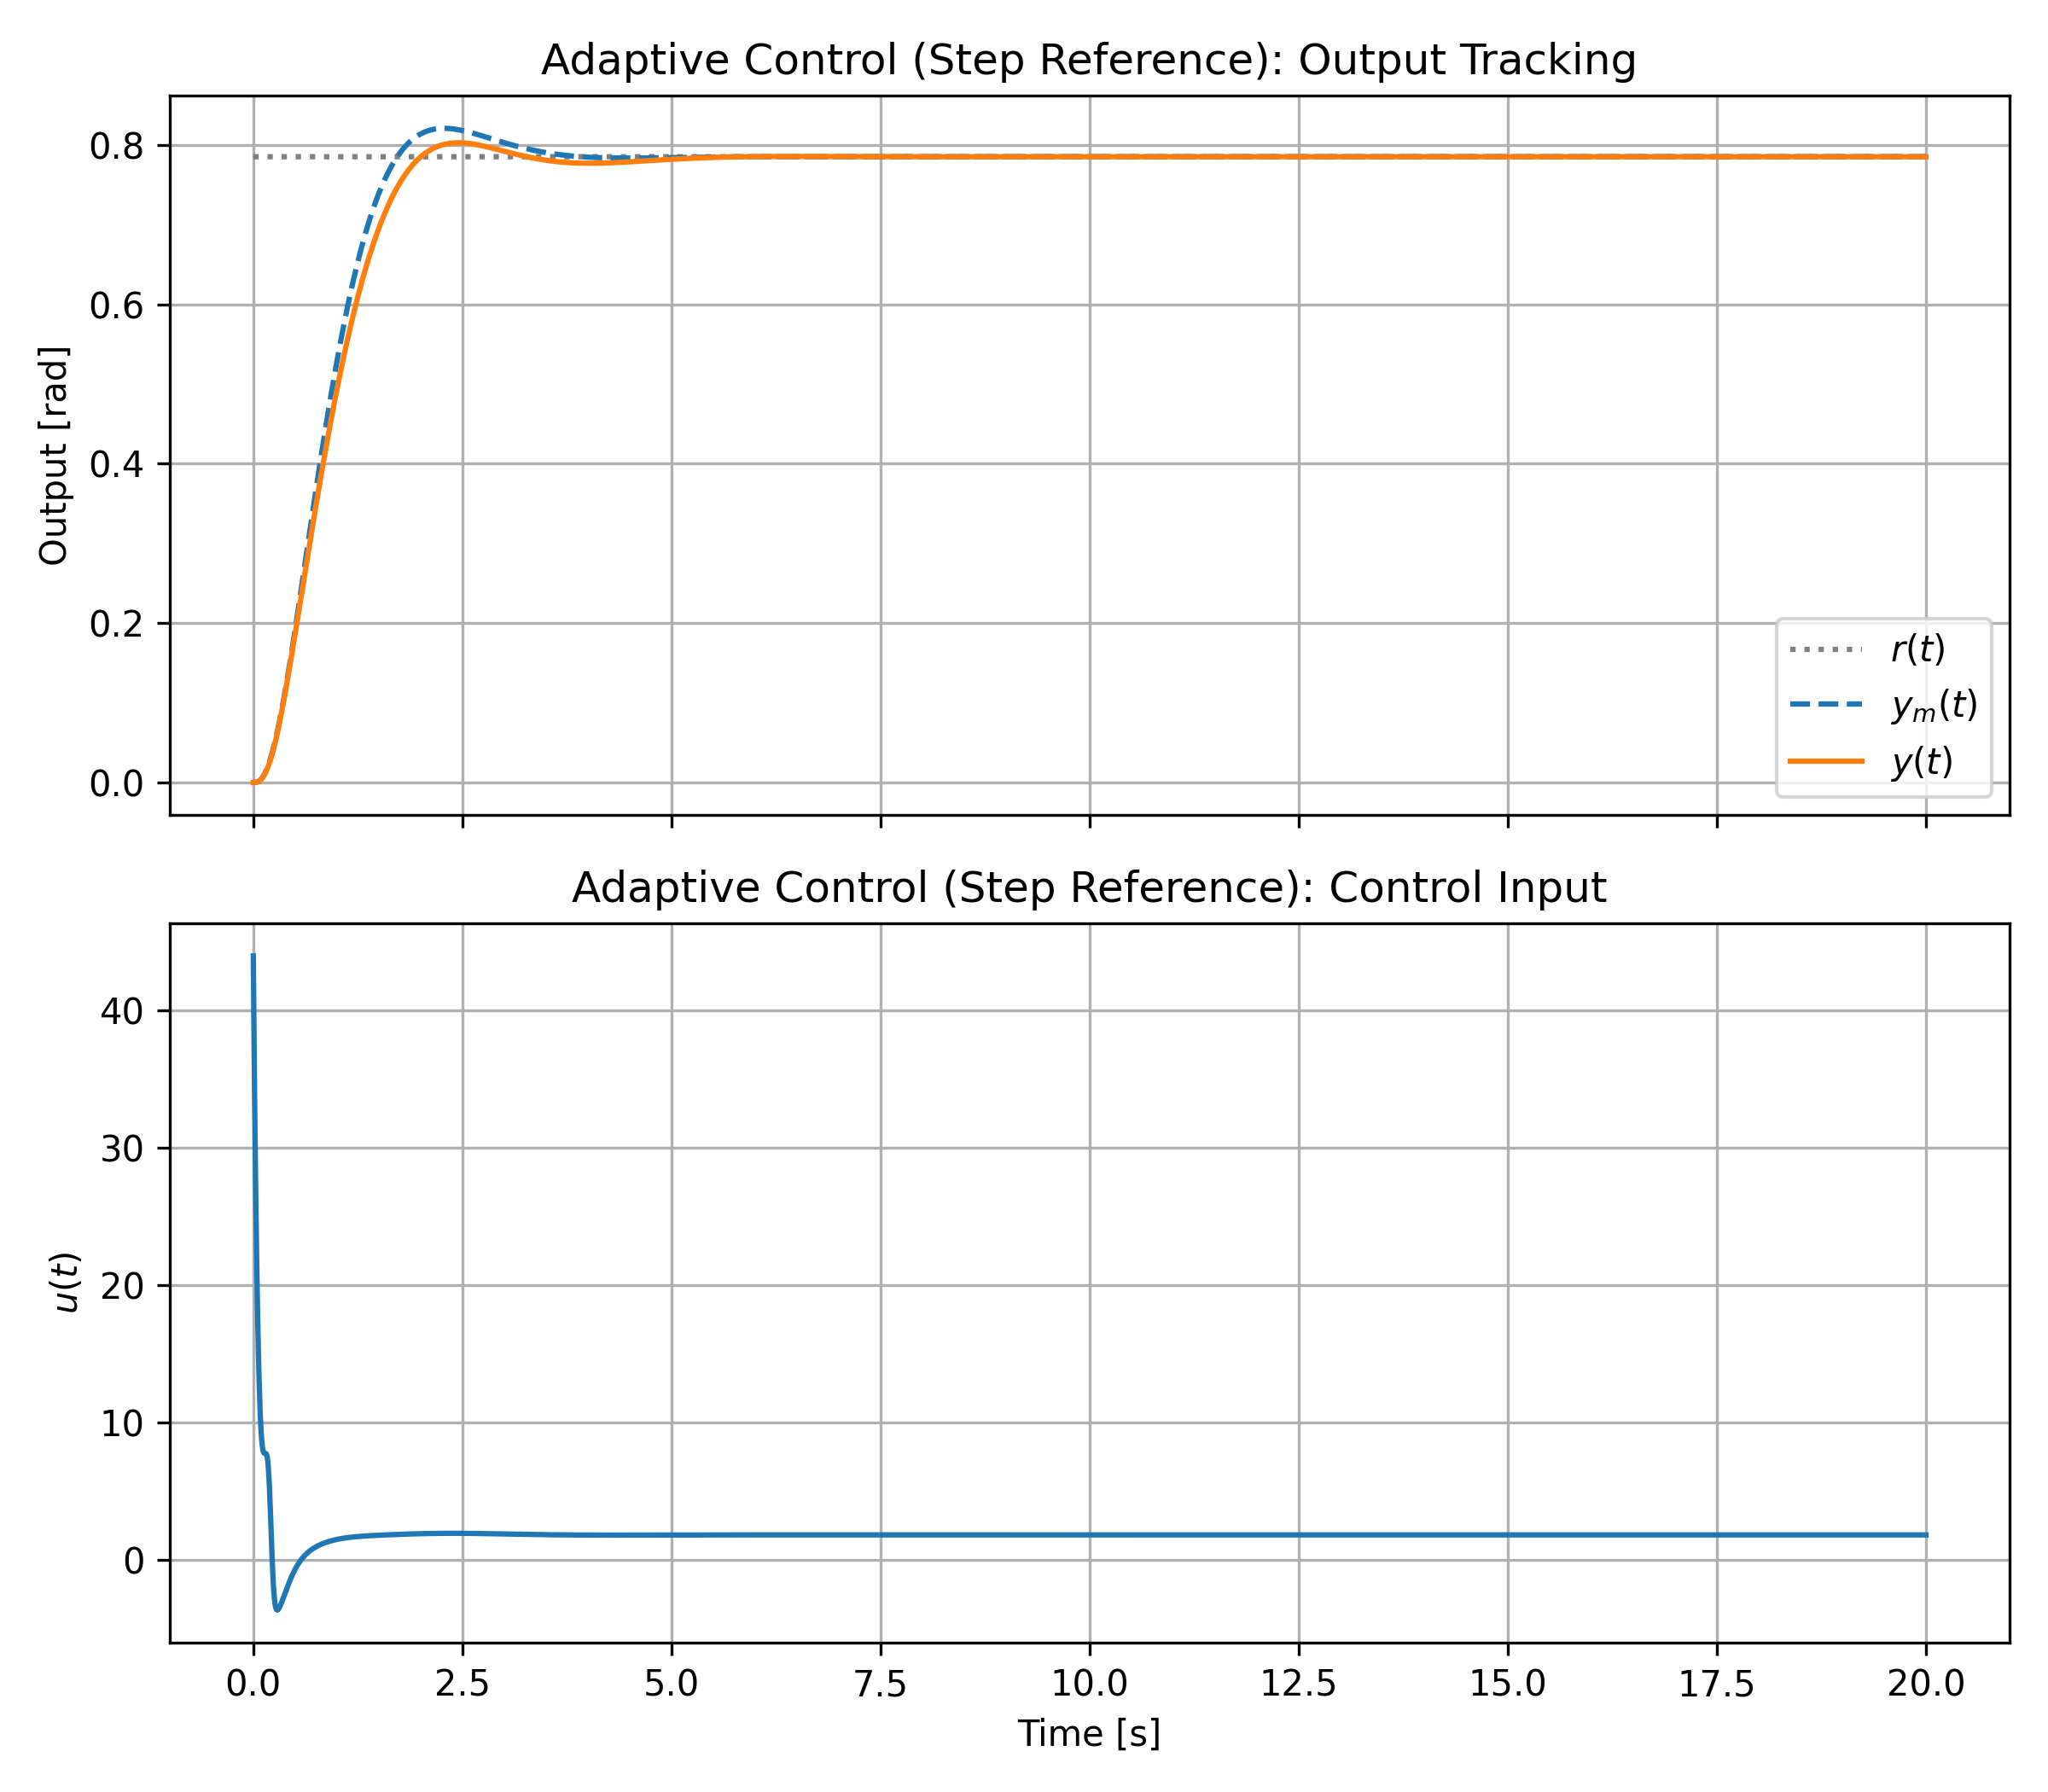
\includegraphics[width=0.65\textwidth]{figs/hw/section4_adaptive_tracking_and_control_step.png}
\caption{Command \(r(t)\), reference model output \(y_m(t)\), and plant output \(y(t)\) (top); Control input \(u(t)\) (bottom).}
\label{fig:adaptive_tracking_and_control_step}
\end{figure}

\begin{figure}[H]
\centering
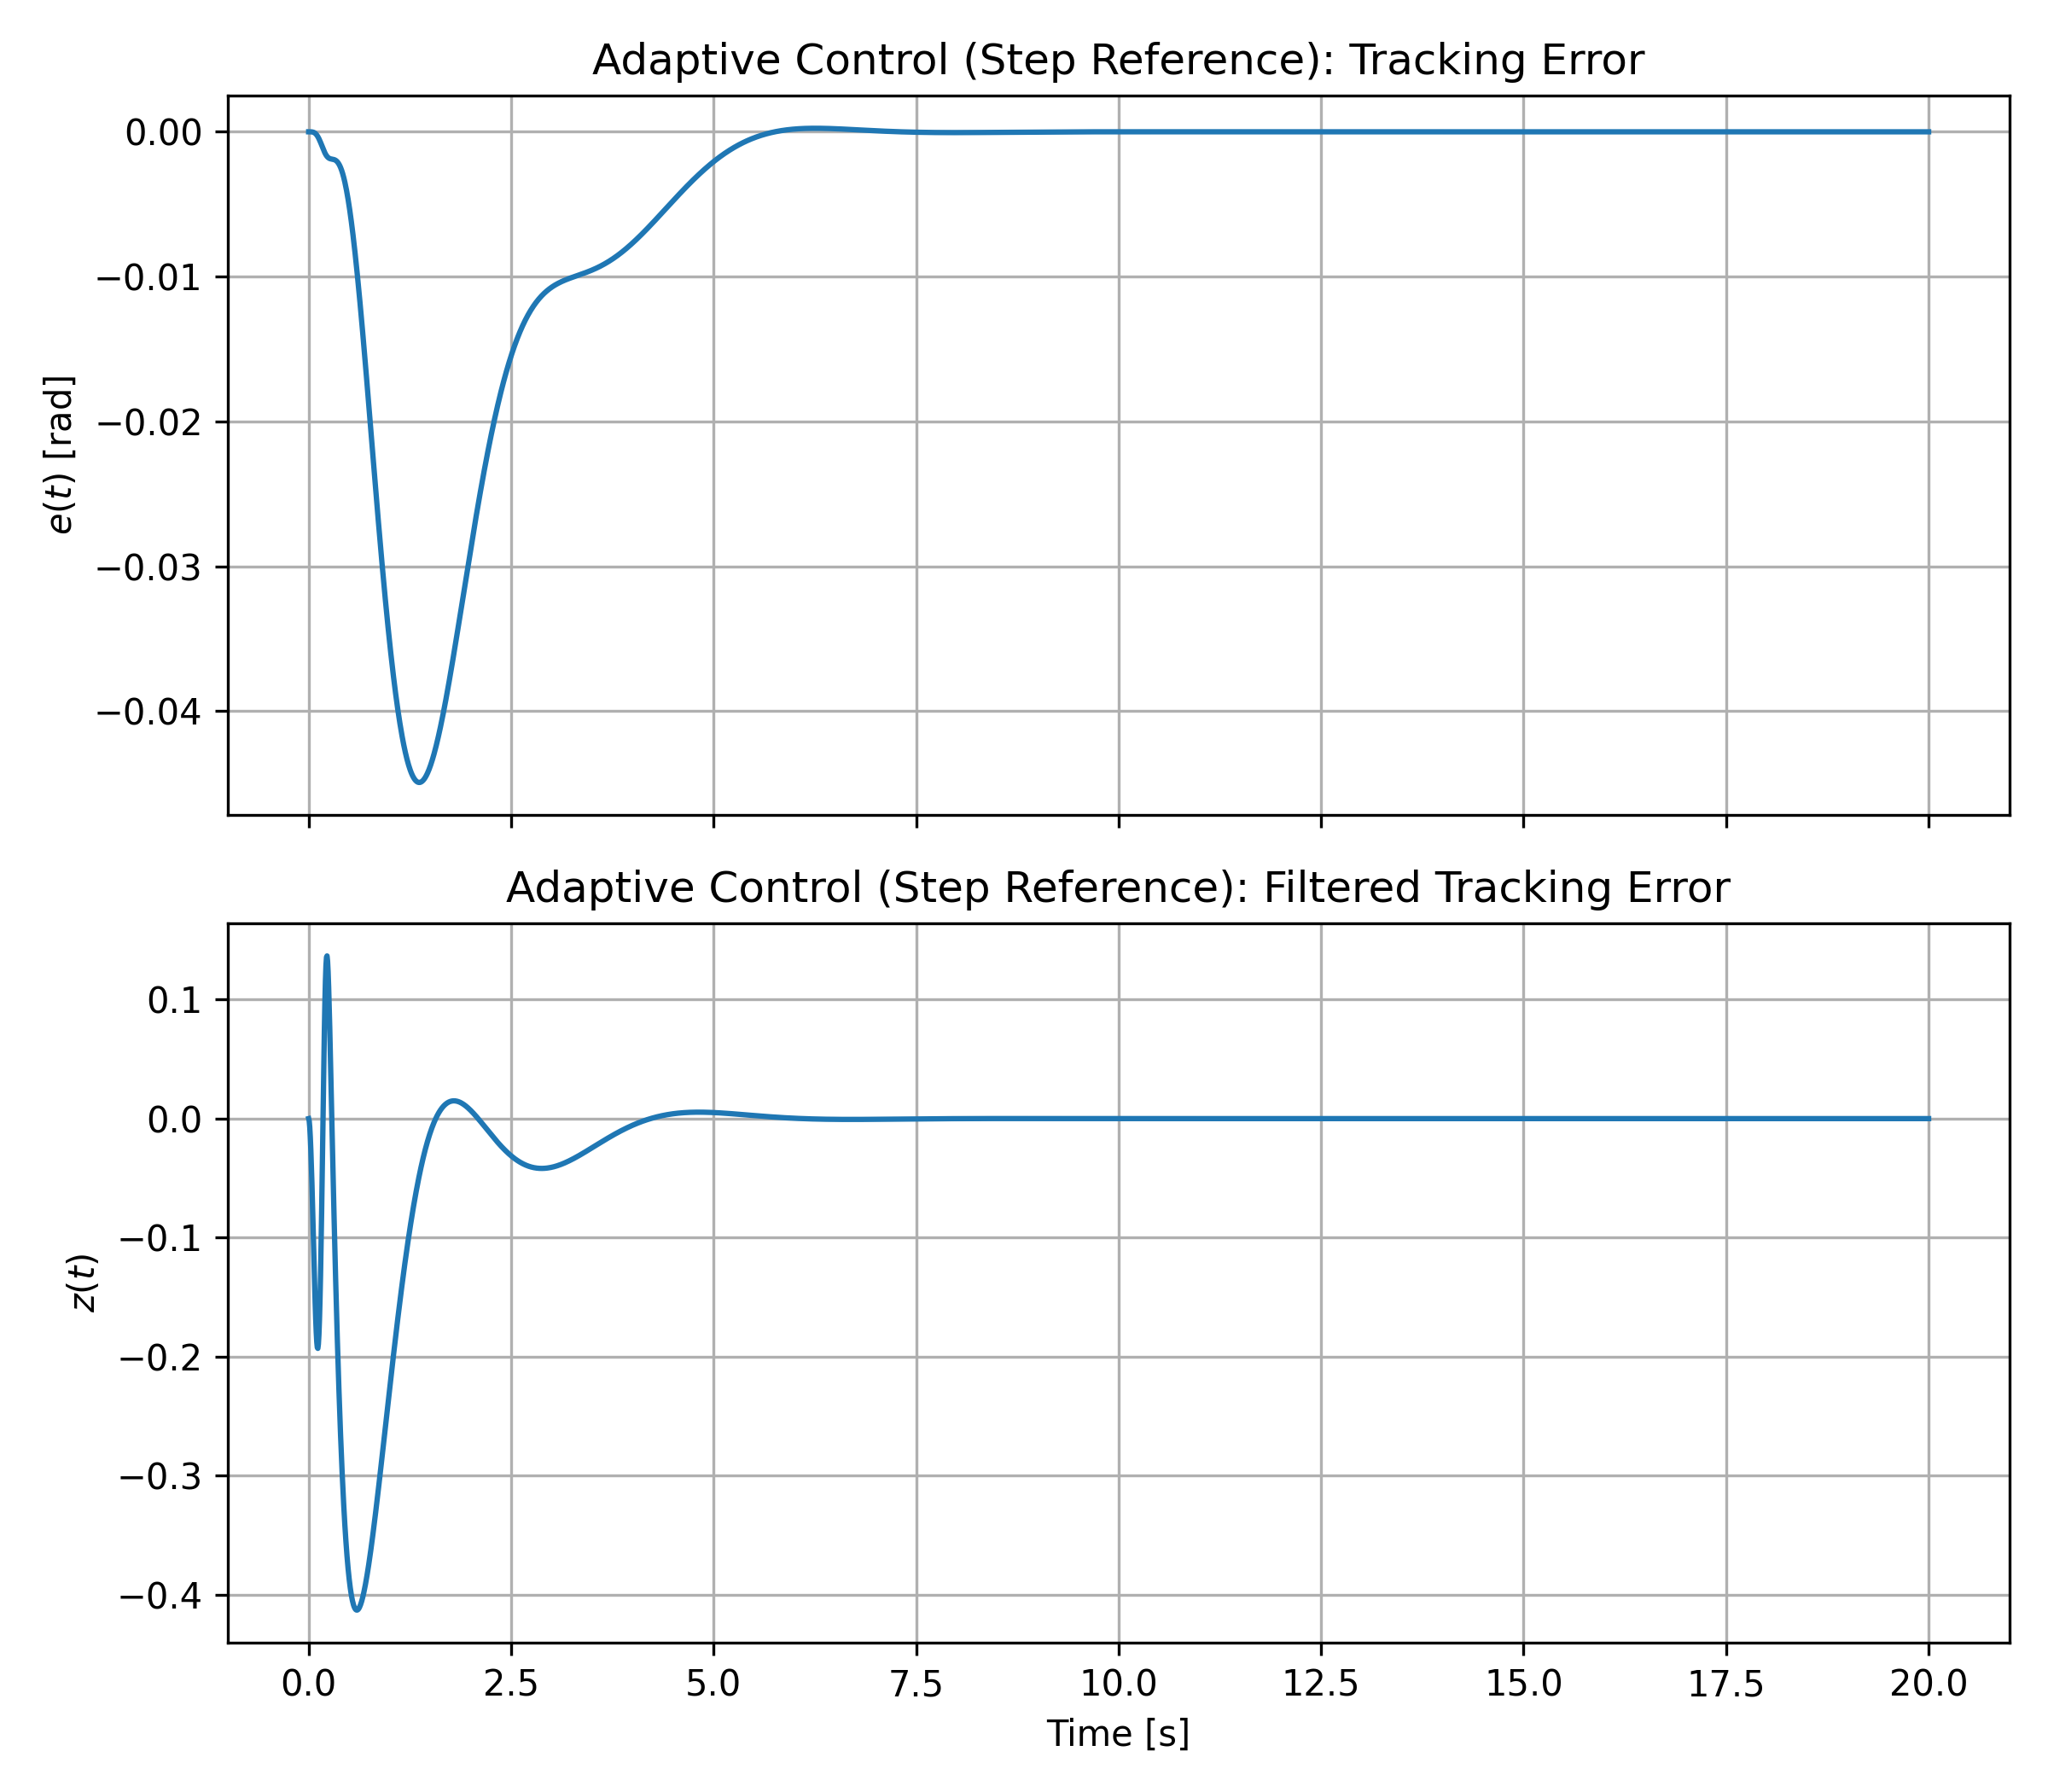
\includegraphics[width=0.65\textwidth]{figs/hw/section4_adaptive_errors_step.png}
\caption{Tracking error \(e(t)\) (top); Filtered tracking error \(z(t)\) (bottom).}
\label{fig:adaptive_errors_step}
\end{figure}

\begin{figure}[H]
\centering
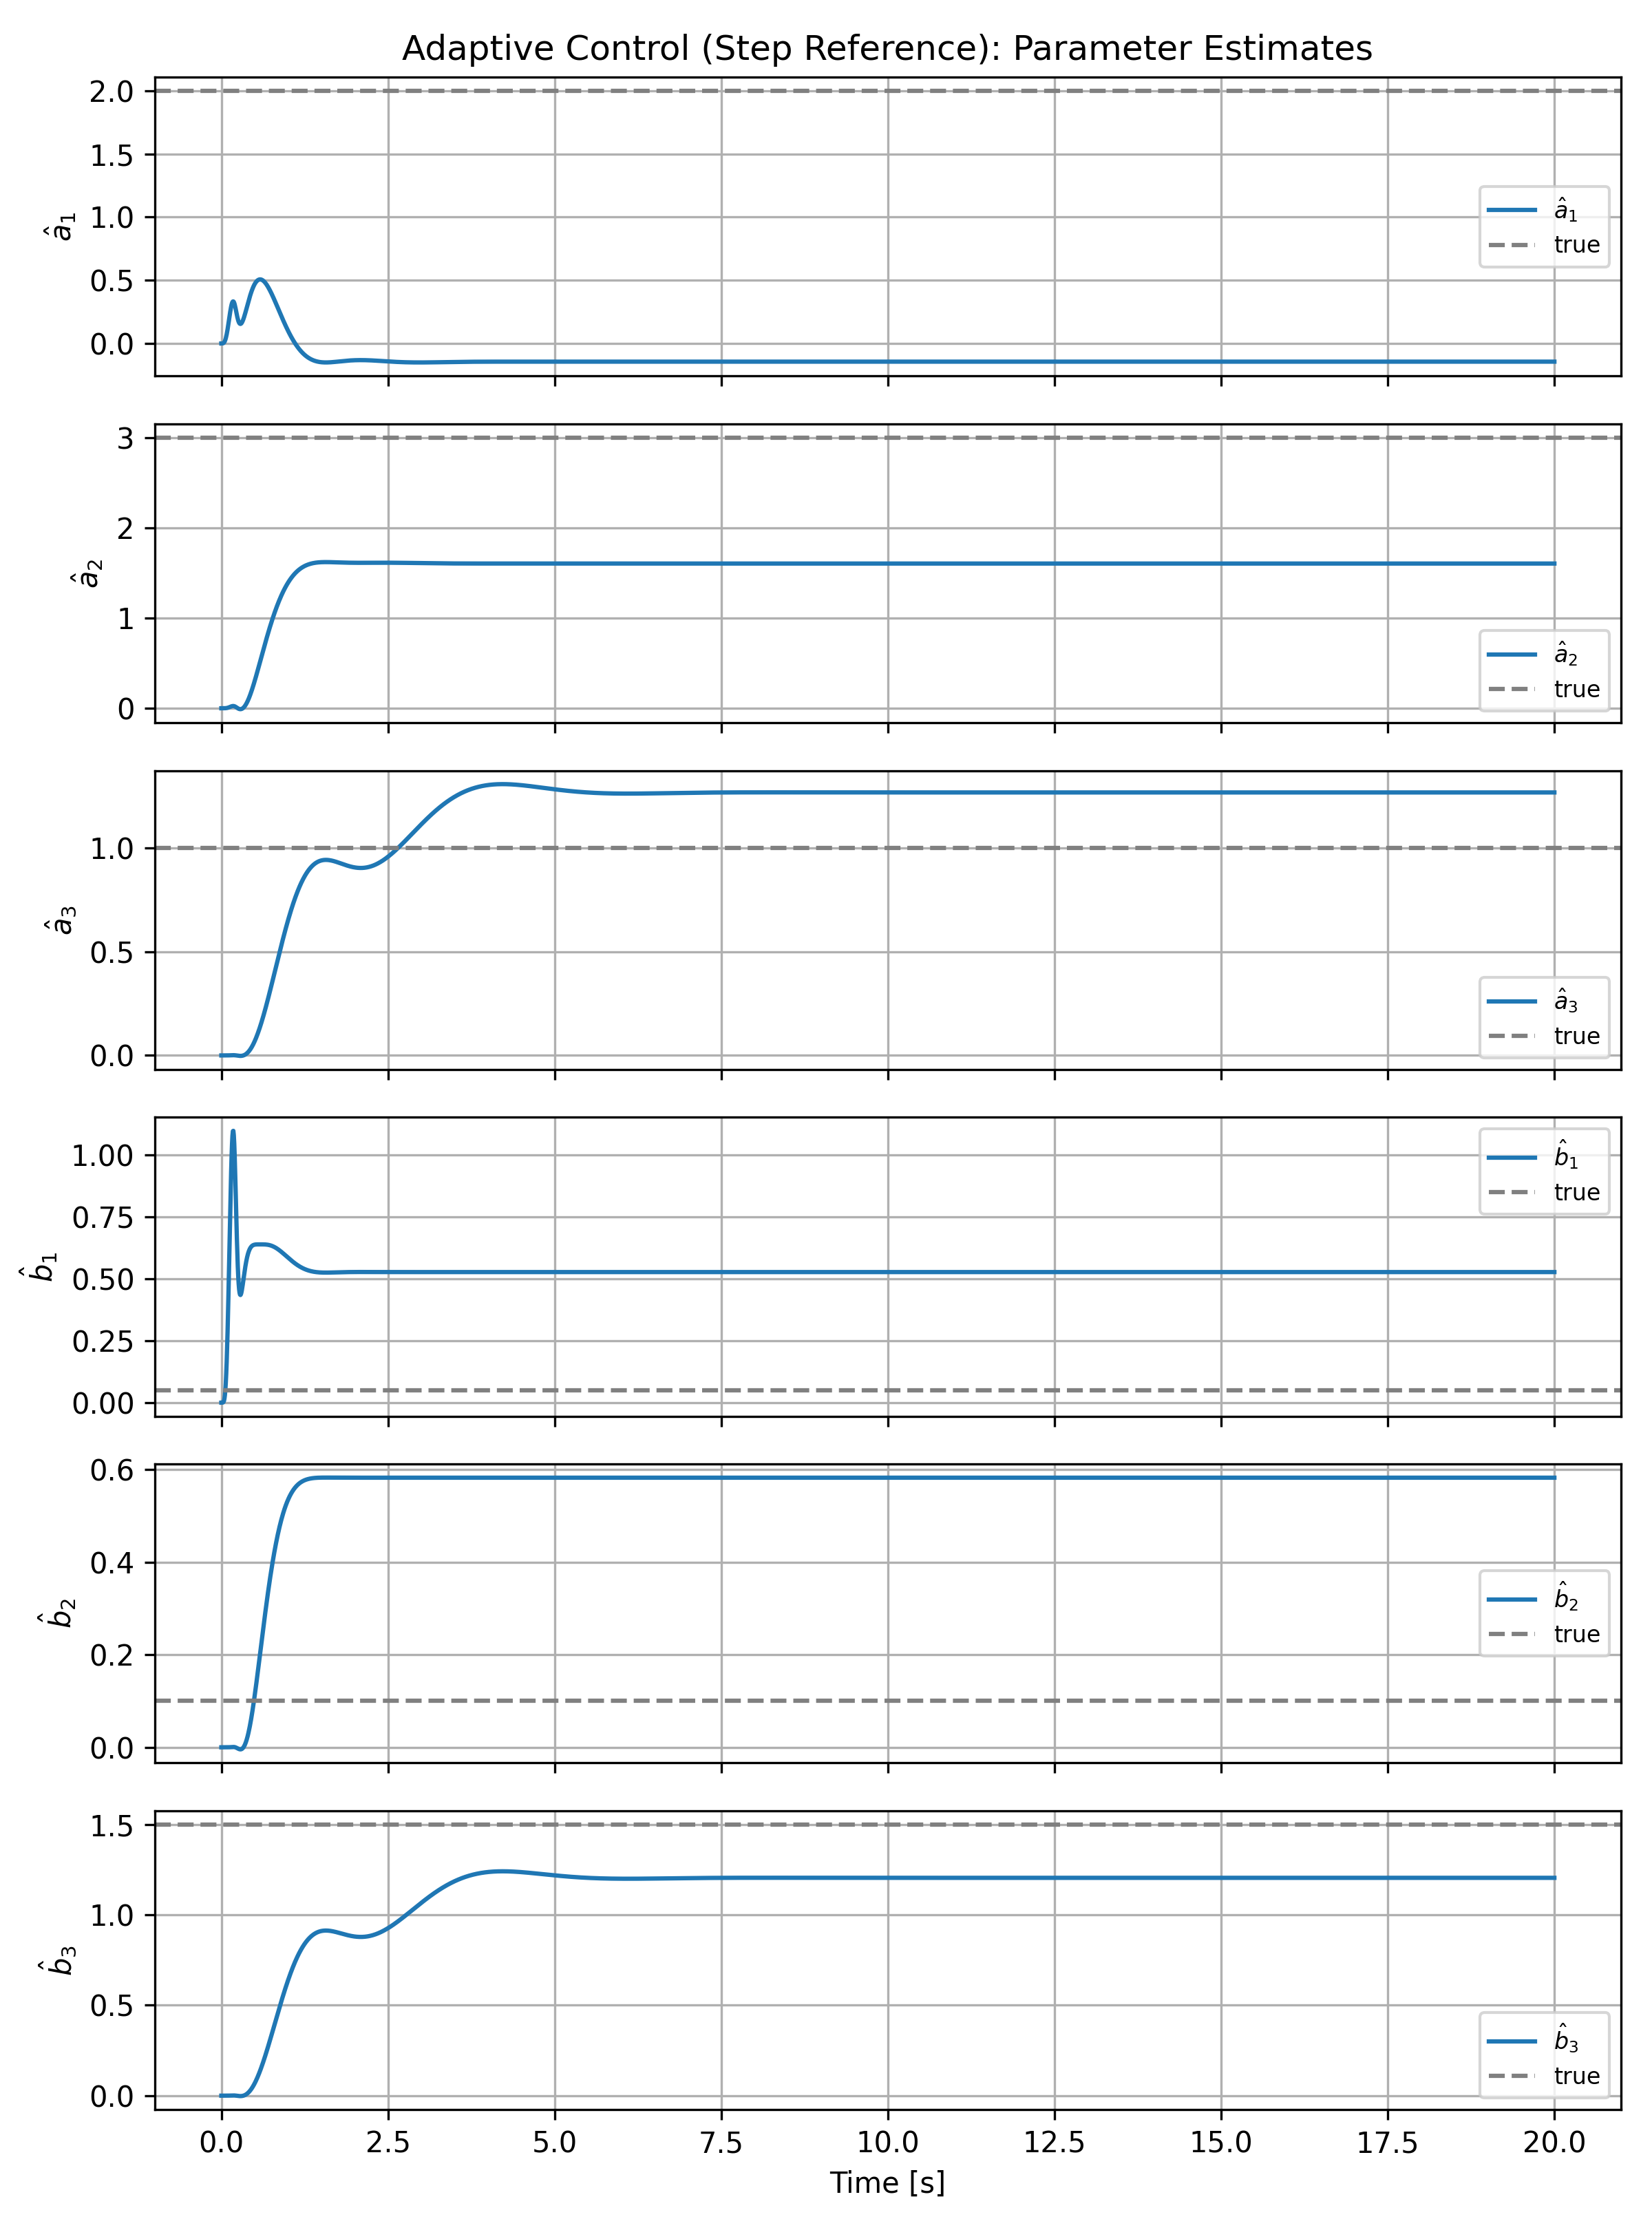
\includegraphics[width=0.7\textwidth]{figs/hw/section4_adaptive_parameter_estimates_step.png}
\caption{Parameter estimates \(\hat{\theta}_i(t)\) vs. True values.}
\label{fig:adaptive_parameter_estimates_step}
\end{figure}

\noindent An important observation is that the parameter estimates do not all converge to their true values. The estimates remain bounded and tracking is achieved, but most components of \(\hat{\theta}\) settle at values noticeably different from \(\theta\). To demonstrate the difference, the same controller is run with the sum-of-sinusoids reference \(r_{\text{PE}}(t)\). The results are shown in figures~\ref{fig:adaptive_tracking_and_control_pe}--\ref{fig:adaptive_parameter_estimates_pe}.

\begin{figure}[H]
\centering
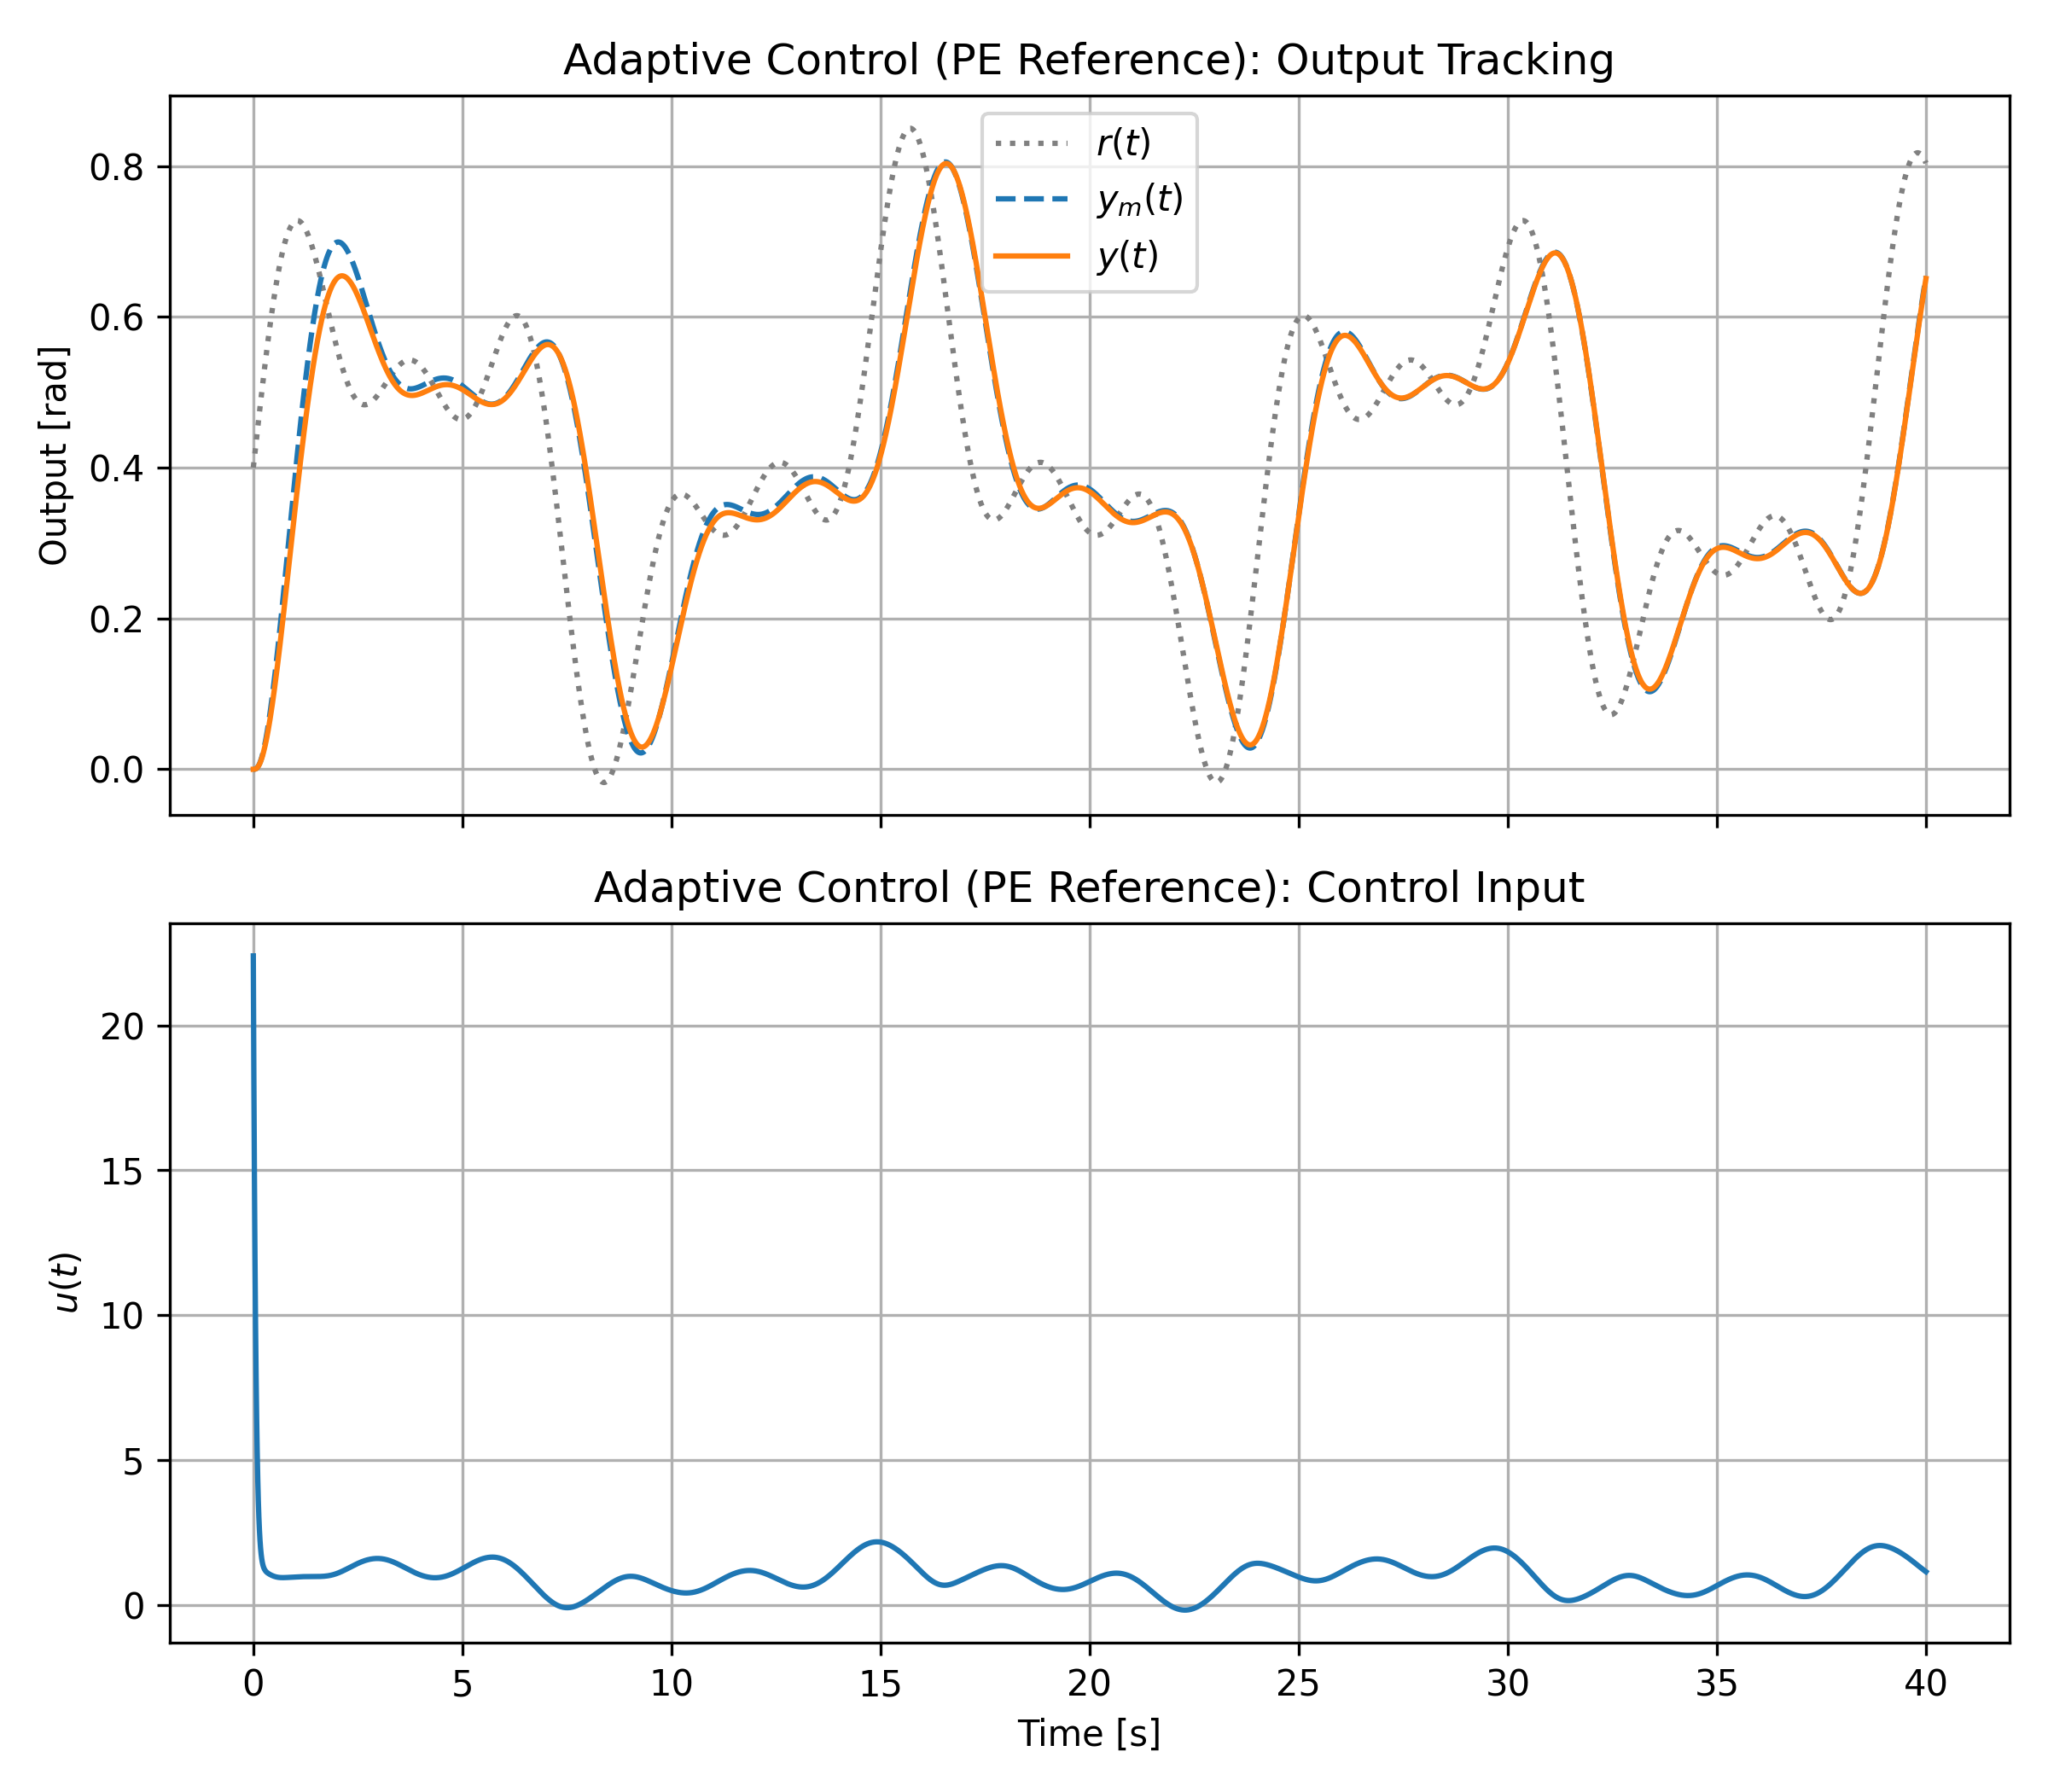
\includegraphics[width=0.7\textwidth]{figs/hw/section4_adaptive_tracking_and_control_pe.png}
\caption{Command \(r(t)\), reference model output \(y_m(t)\), and plant output \(y(t)\) (top) ; Control input \(u(t)\) (bottom).}
\label{fig:adaptive_tracking_and_control_pe}
\end{figure}

\begin{figure}[H]
\centering
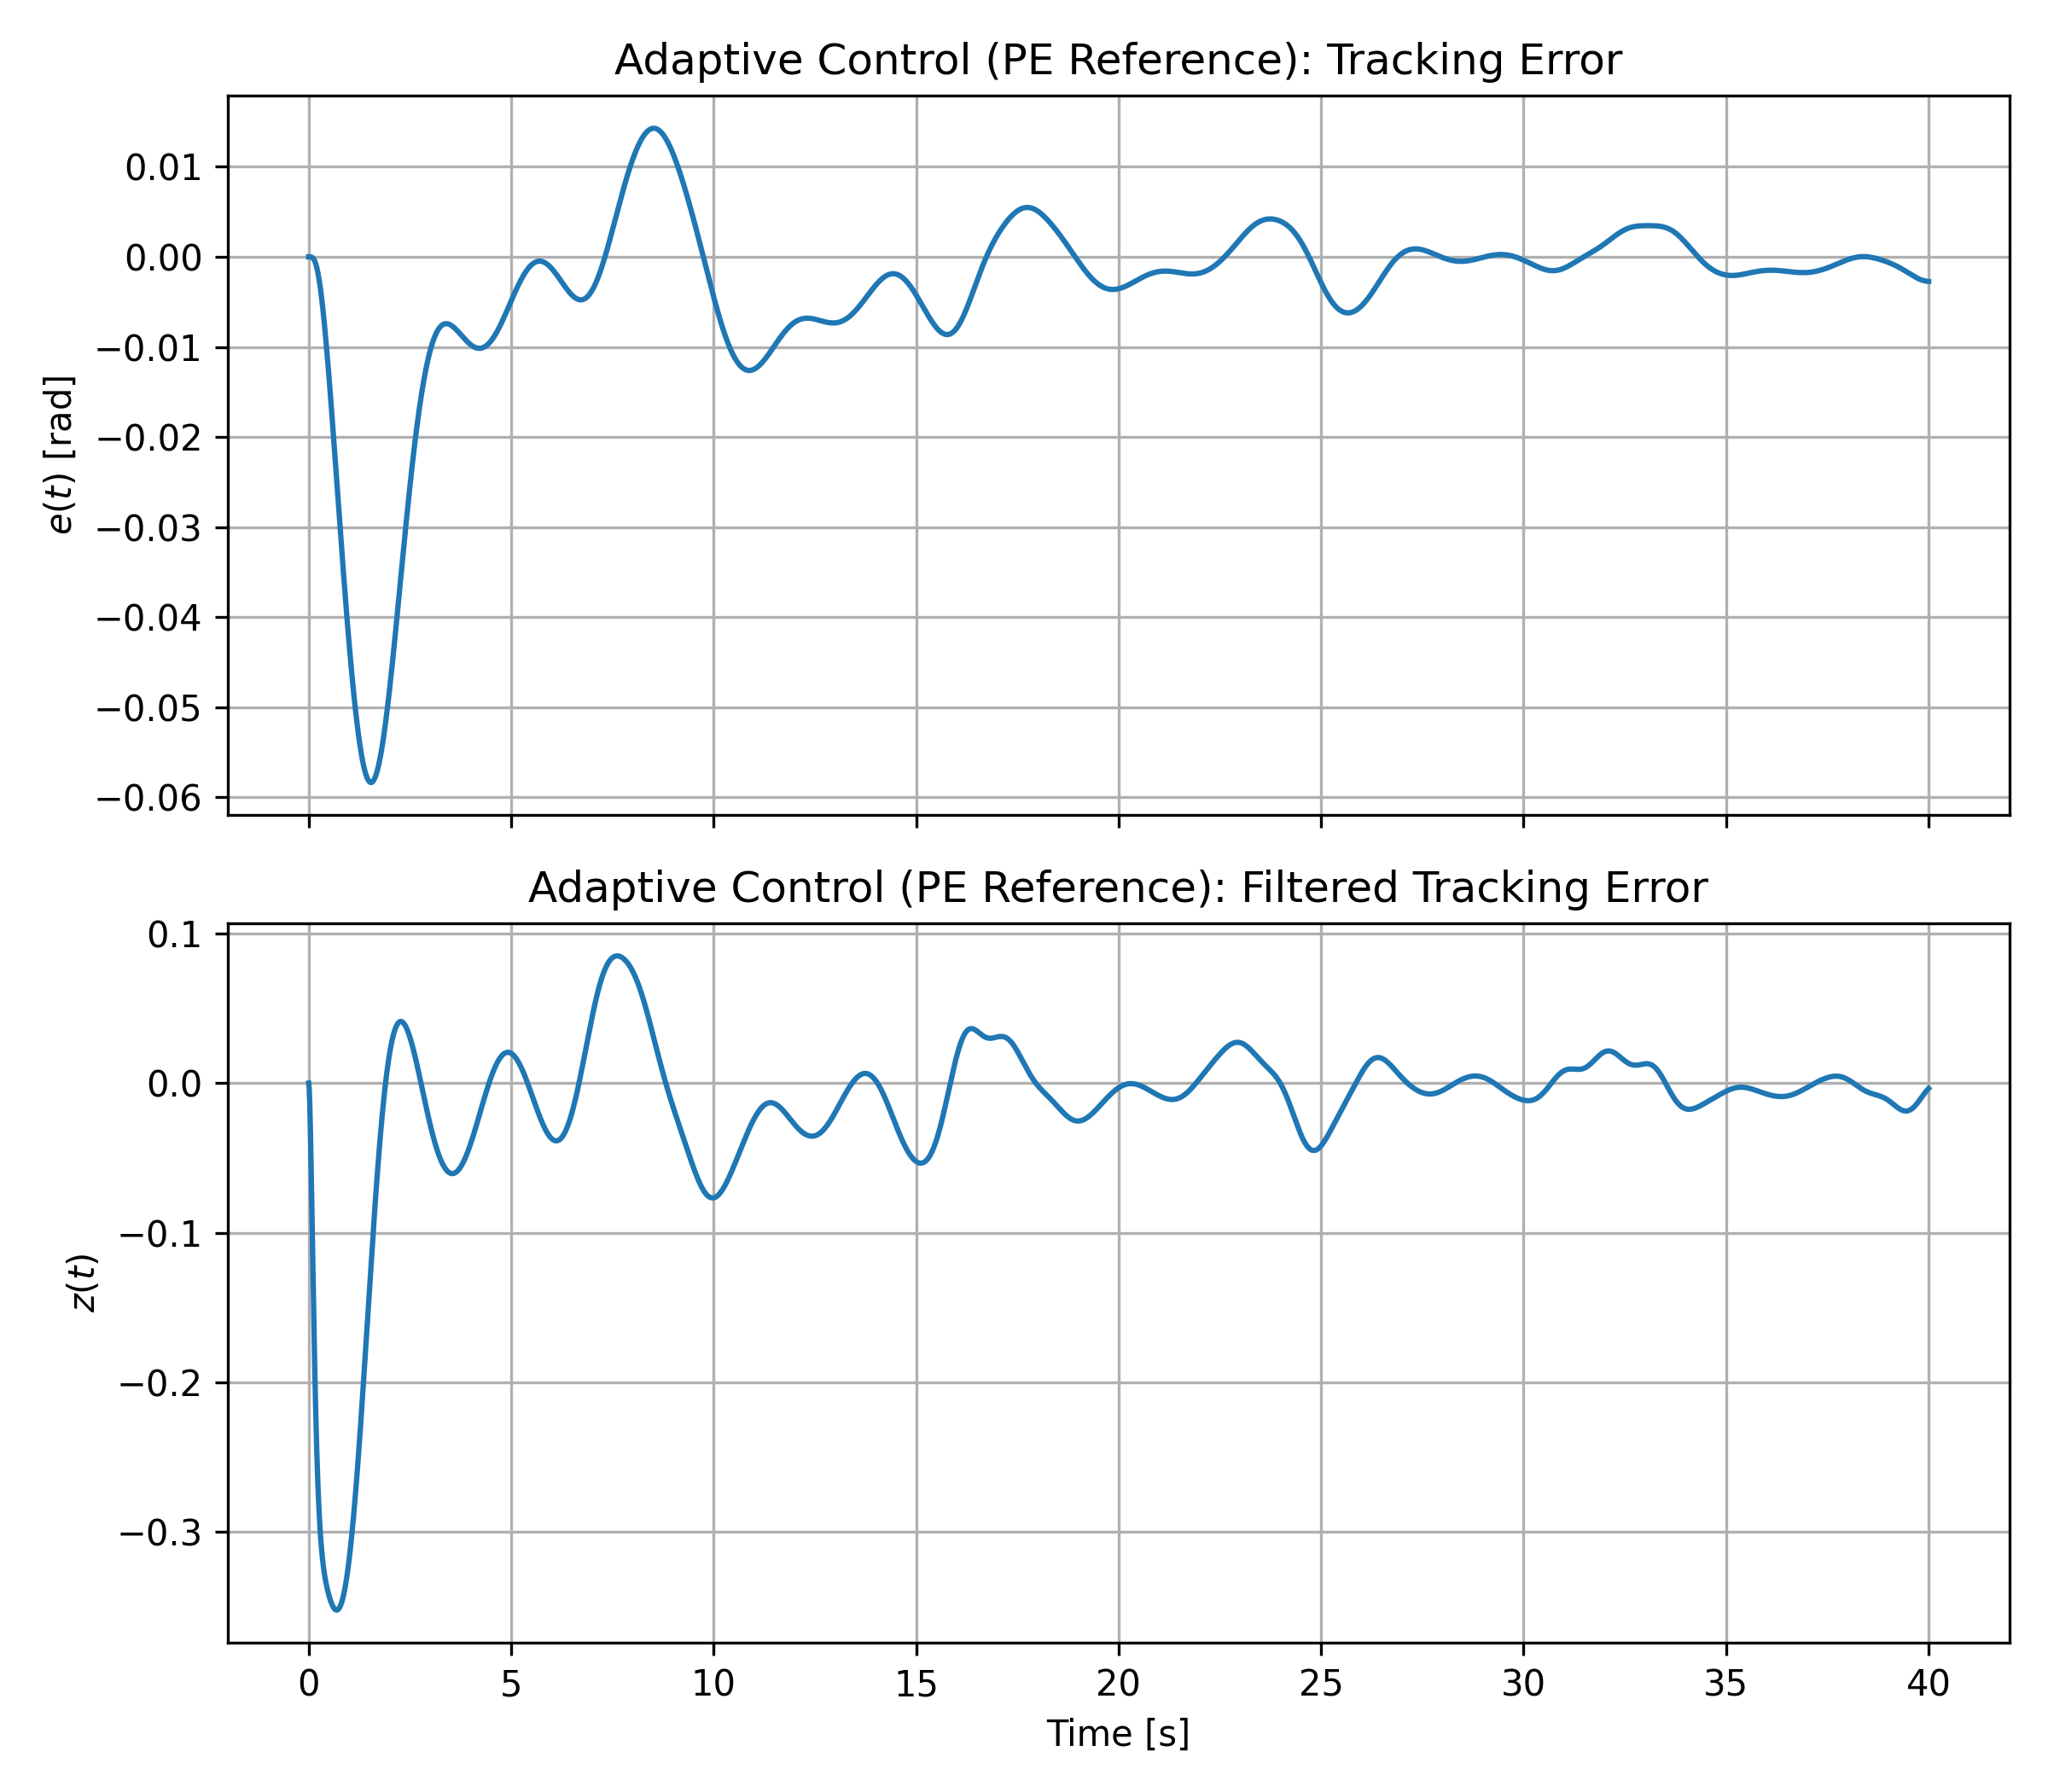
\includegraphics[width=0.7\textwidth]{figs/hw/section4_adaptive_errors_pe.png}
\caption{Tracking error \(e(t)\) (top);Filtered tracking error \(z(t)\) (bottom).}
\label{fig:adaptive_errors_pe}
\end{figure}

\begin{figure}[H]
\centering
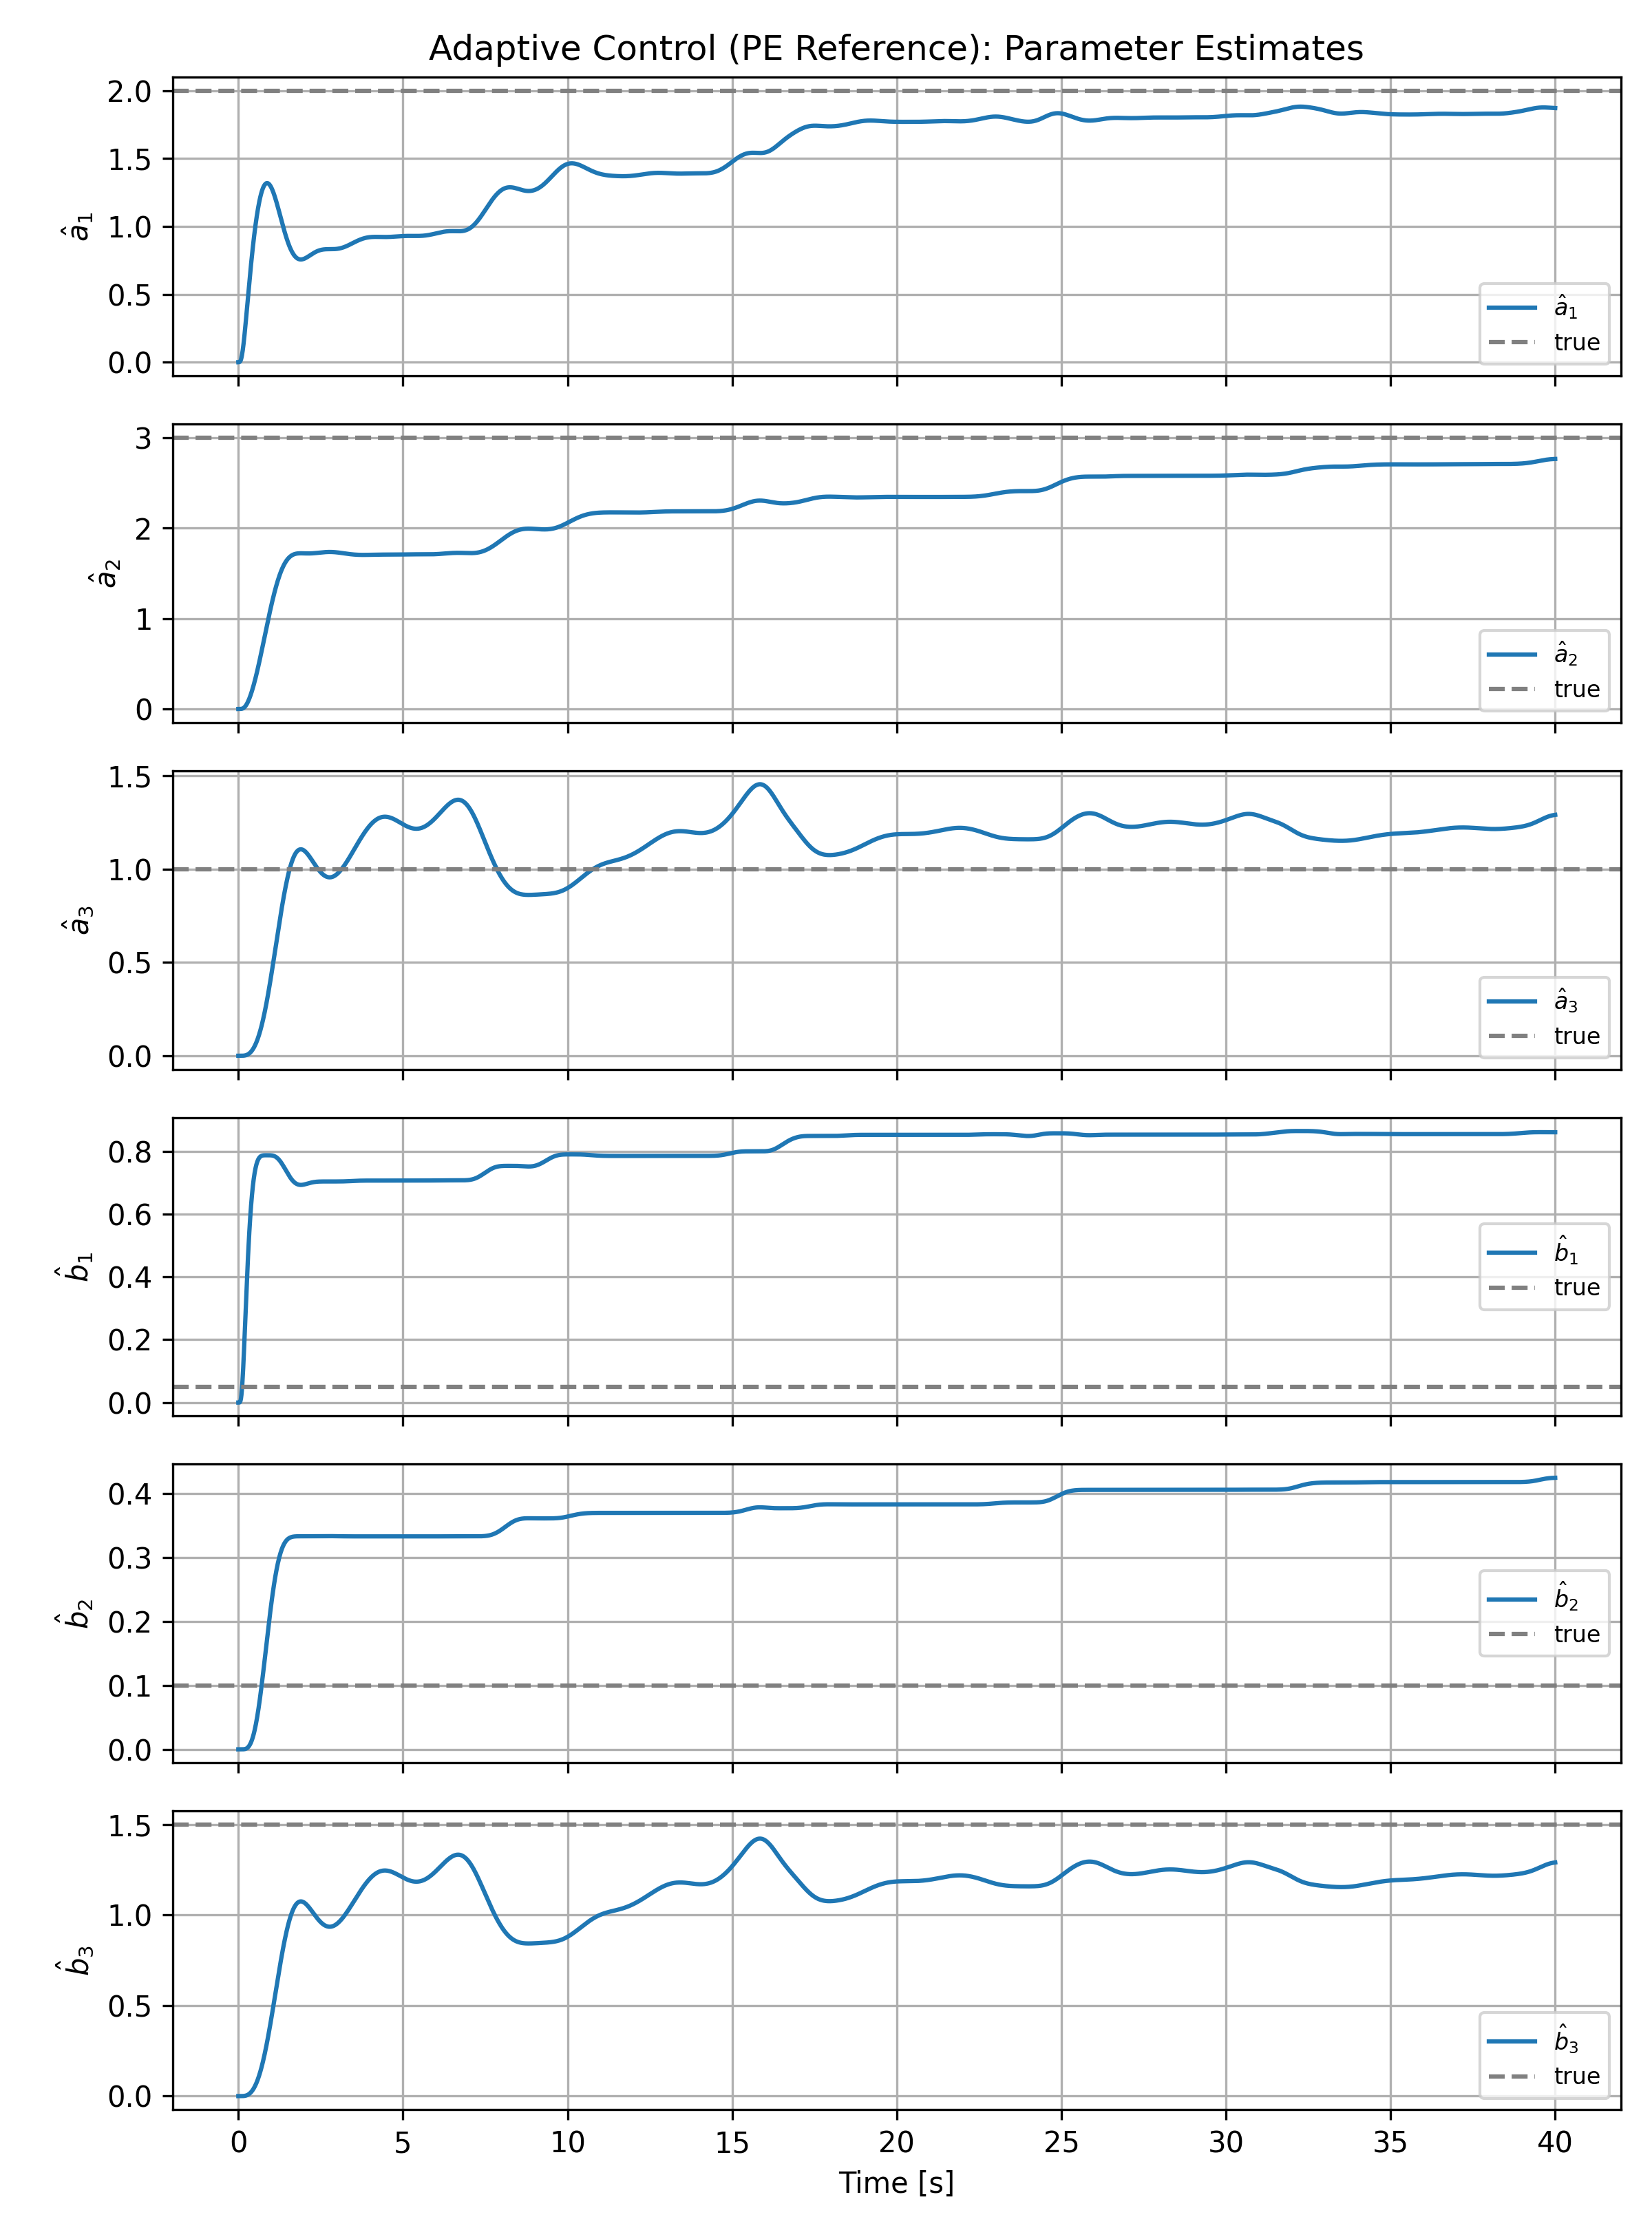
\includegraphics[width=0.7\textwidth]{figs/hw/section4_adaptive_parameter_estimates_pe.png}
\caption{Parameter estimates \(\hat{\theta}_i(t)\) vs. True values.}
\label{fig:adaptive_parameter_estimates_pe}
\end{figure}

\noindent The adaptive controller successfully achieved the main control objective in both simulations. Even though the plant parameters were initially unknown, the controller maintained stability and the plant output tracked the reference model output.
For the step input, the tracking error converged to zero, but the parameter estimates did not converge to their true values. This occurred because the constant reference signal did not sufficiently excite all parts of the system. As a result, the controller learned enough information to achieve accurate tracking, but not enough to uniquely identify all model parameters.
In the sum-of-sinusoid case, the parameter estimates converged much closer to their true values while maintaining good tracking performance.
To recover the true plant parameters, the reference signal must provide sufficient excitation.

\bigskip
